\documentclass[main.tex]{subfiles}

\begin{document}

\chapter{Post Assembly} 

Assemblies tools try to reduce information to speed up assembly, if we have less reads we take less time to found overlap if we have less overlap, assembly graph can feet in memory and her cleaning take less time. All assembly pipeline we describe in previous chapter use heursitics to reduce the quantity of information they have to use to find the assembly solution. This heuristics was generaly are careful and didn't remove important information but for some case this heuristics failled.

Some times the heursitics failled and they remove an important read/overlap the assembly was fragmented. In many case long-read assembly was fragmented when a repetition isn't span by a reads, but in some case repetition can't explain fragmentation. Figure \ref{postassembly:fig:t_roseus_example} present an example on a assembly of Pacbio like synthetic dataset generate by LongISLND\cite{longislnd} and assembled by \canu, this assembly contains three contigs and one of fragmentation can't be explain by a repetition.

\begin{figure}[ht]
    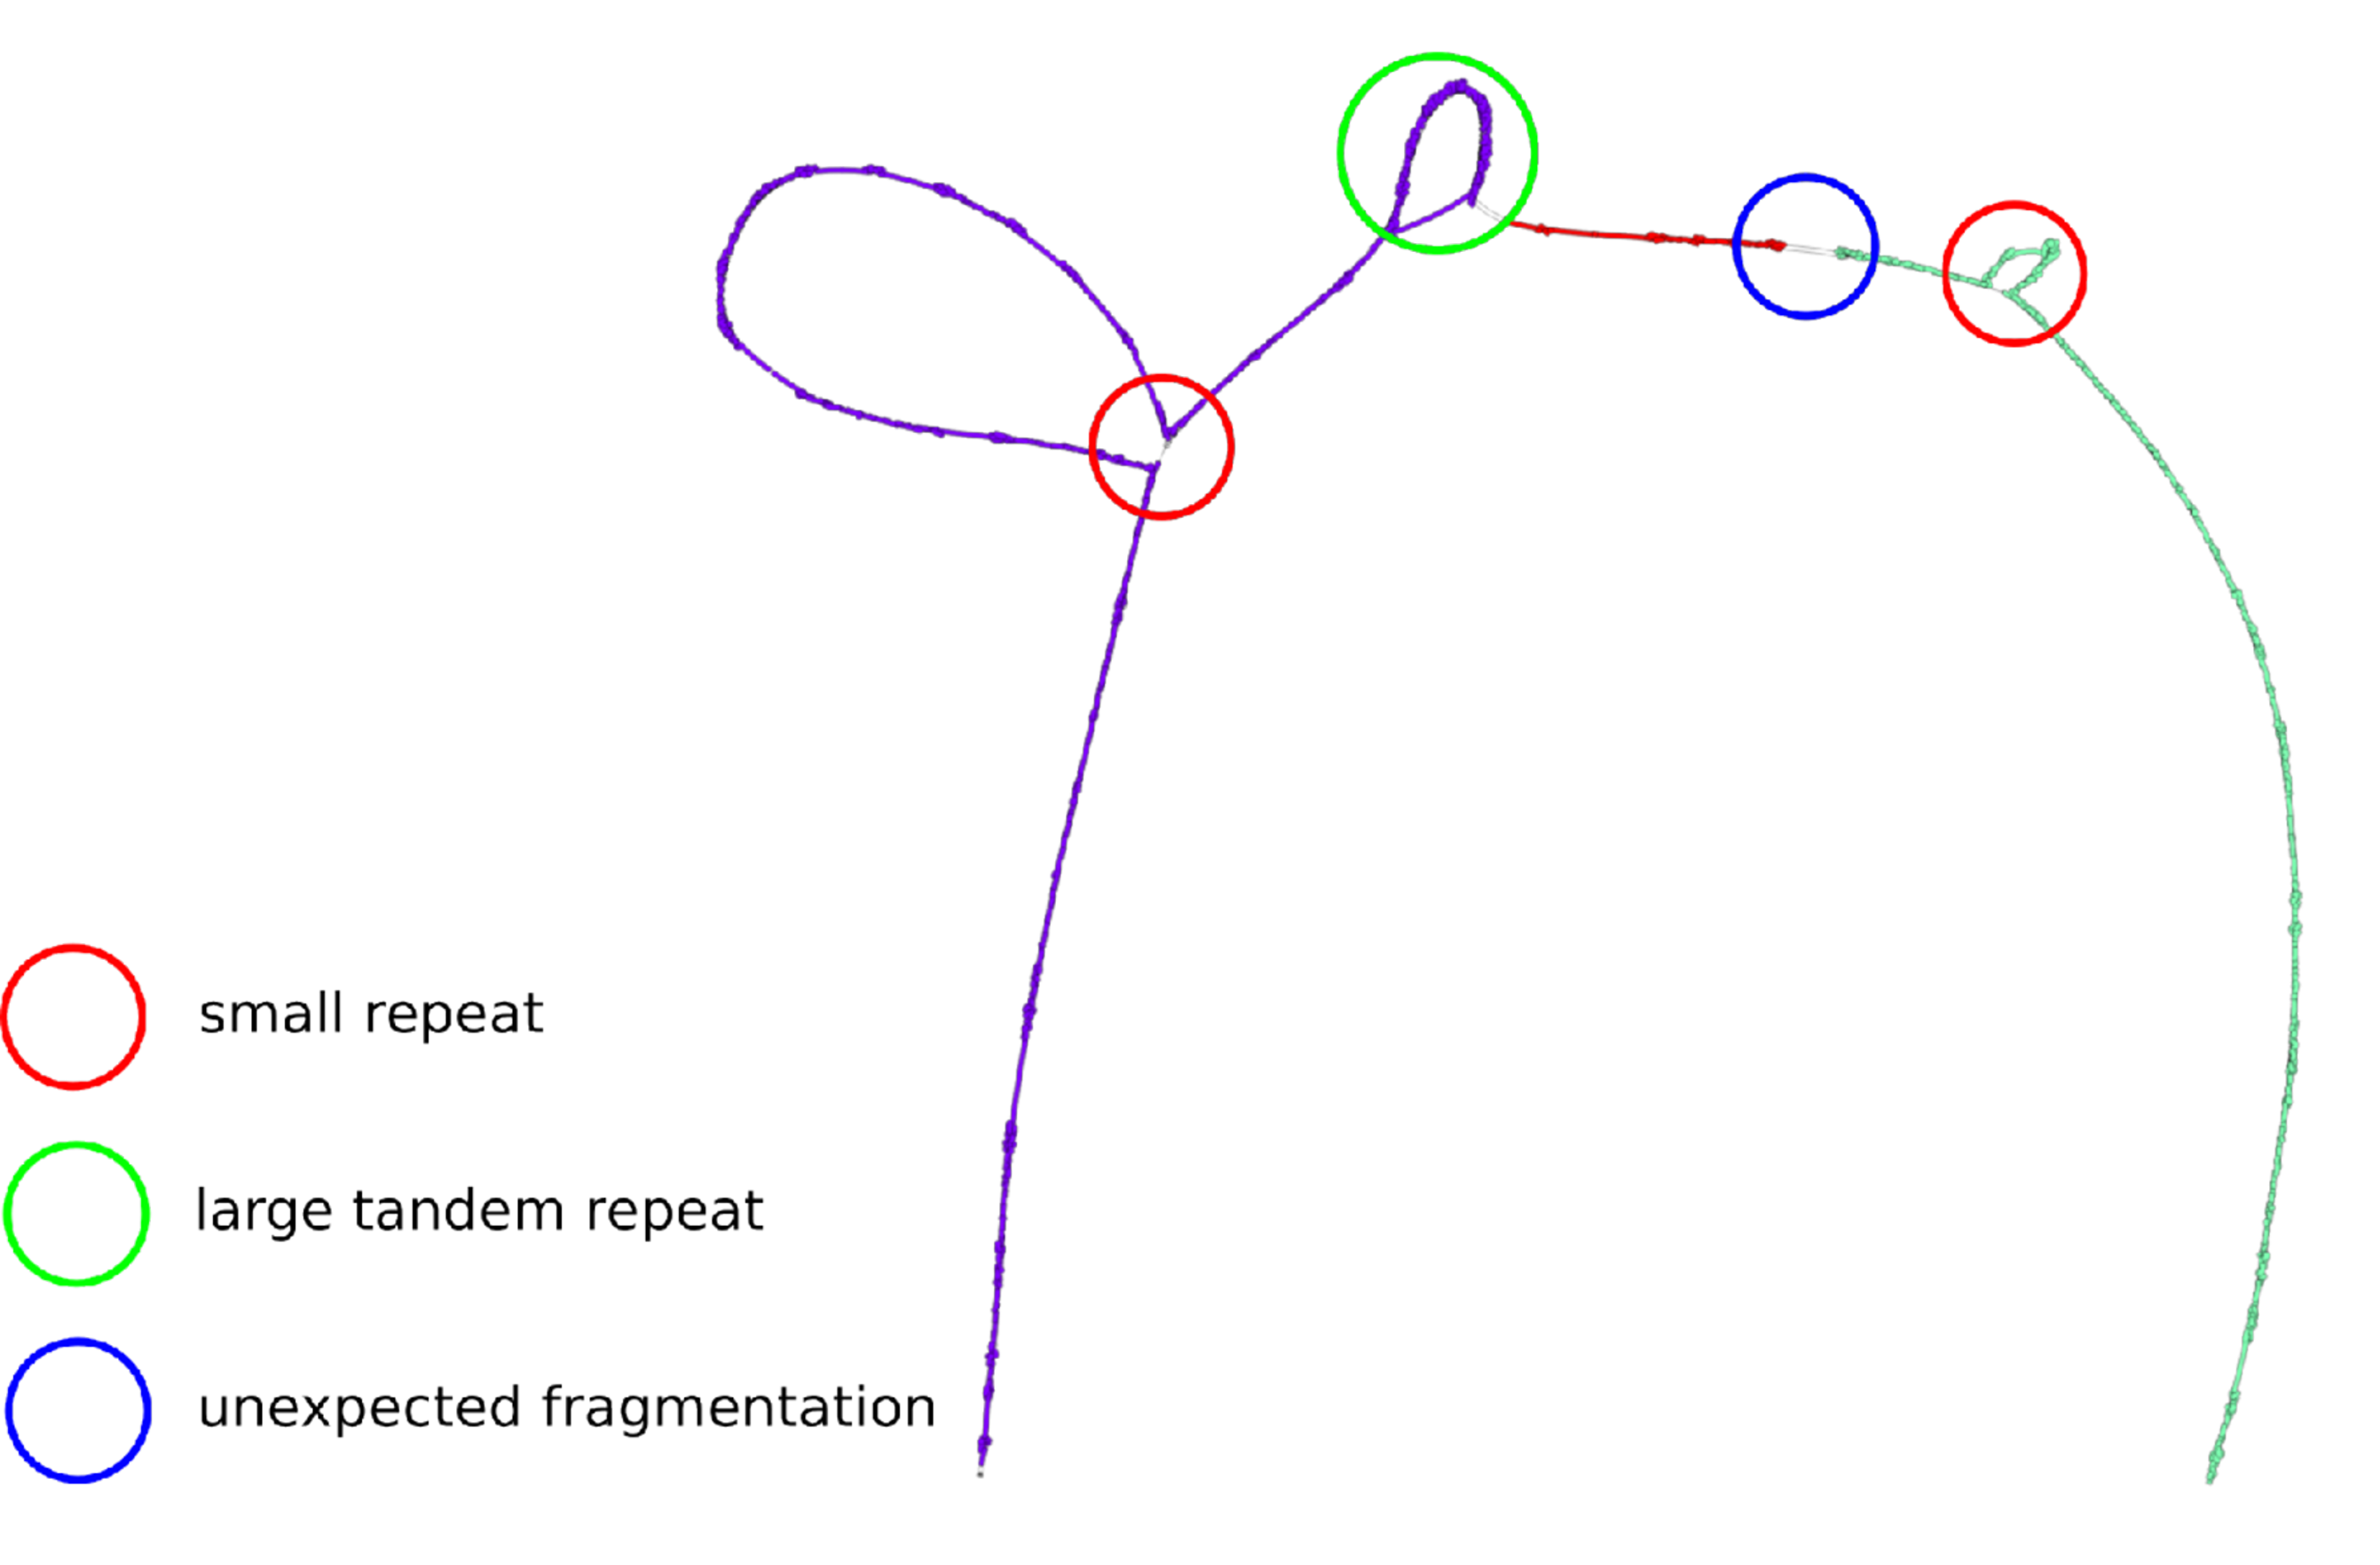
\includegraphics[width=\textwidth]{postassembly/images/t_roseus_projection_annoted.pdf}
    \caption{This graph was the overlap graph (found by \minimap), read used by \canu to build a contigs was are colored with same color. We can observe 2 fragmentation point, one can be explain by a repetition, green circle, we can observe repetition solved by \canu, but the fragmentation between green and red can't be explain by a repetition.}
    \label{postassembly:fig:t_roseus_example}
\end{figure}

In Figure \ref{postassembly:fig:t_roseus_example} in fact we present the main idea of \knot combine information of assembly (the read coloration) with a maximum of information can be extract from reads (the \OLC graph build from \minimap). The information from contigs help us to ignore some already solve problem (red circle), unsolvable trouble (greed circle), to focus on strange situation (blue circle). Figure \ref{postassembly:fig:t_roseus_example} show a very simple example in real case the \OLC graph cann't be readable. For thes reason and to run analysis without an human eye we automatise the idea of \knot in a simple tools.

The paper was publish originally publish in Bioinformatics (\url{https://doi.org/10.1093/bioinformatics/btz219}), we reformat the paper in the style of this current document for reasons of readability.

\subfile{paper/knot.tex}


\section{Conclusion}

In this paper we show the idea to go back to raw read information, could be very help full for bacterial assembly. To use \knot on more complex dataset we need improve some part of \knot, especially the construction of the graph, its representation in memory and the search of paths between contigs extremity. This improvement required some code writing, but the original idea of comme back to raw read information can be used for more genome assembly improvement. I present this idea, in my conclusion.


\onlyinsubfile{
\bibliographystyle{plainnat}
\bibliography{main}
\addcontentsline{toc}{chapter}{Bibliography}
}

\end{document}